\documentclass[a4paper, 12pt]{article}
% packages
\usepackage{amssymb}
\usepackage[fleqn]{mathtools}
\usepackage{tikz}
\usepackage{enumerate}
\usepackage{bussproofs}
\usepackage{xcolor}
\usepackage[margin=1.3cm]{geometry}
\usepackage{logicproof}
\usepackage{diagbox}
\usepackage{listings}
\usepackage{graphicx}
\usepackage{lstautogobble}
\usepackage{hyperref}
\usepackage{multirow}
\usetikzlibrary{arrows, shapes.gates.logic.US, circuits.logic.US, calc, automata, positioning}

% shorthand for verbatim
% this clashes with logicproof, so maybe fix this at some point?
\catcode`~=\active
\def~#1~{\texttt{#1}}

% code listing
\lstdefinestyle{main}{
    numberstyle=\tiny,
    breaklines=true,
    showspaces=false,
    showstringspaces=false,
    tabsize=2,
    numbers=left,
    basicstyle=\ttfamily,
    columns=fixed,
    fontadjust=true,
    basewidth=0.5em,
    autogobble,
    xleftmargin=3.0ex,
    mathescape=true
}
\newcommand{\dollar}{\mbox{\textdollar}} %
\lstset{style=main}

% augmented matrix
\makeatletter
\renewcommand*\env@matrix[1][*\c@MaxMatrixCols c]{%
\hskip -\arraycolsep
\let\@ifnextchar\new@ifnextchar
\array{#1}}
\makeatother

% ceiling / floor
\DeclarePairedDelimiter{\ceil}{\lceil}{\rceil}
\DeclarePairedDelimiter{\floor}{\lfloor}{\rfloor}

% custom commands
\newcommand{\indefint}[2]{\int #1 \, \mathrm{d}#2}
\newcommand{\defint}[4]{\int_{#1}^{#2} #3 \, \mathrm{d}#4}
\newcommand{\dif}[2]{\frac{\mathrm{d}#1}{\mathrm{d}#2}}
\newcommand{\limit}[2]{\raisebox{0.5ex}{\scalebox{0.8}{$\displaystyle{\lim_{#1 \to #2}}$}}}
\newcommand{\summation}[3]{\sum\limits_{#1}^{#2} #3}
\newcommand{\intbracket}[3]{\left[#3\right]_{#1}^{#2}}
\newcommand{\ulsmash}[1]{\underline{\smash{#1}}}

\newcommand{\powerset}[0]{\wp}
\renewcommand{\emptyset}[0]{\varnothing}
\newcommand{\la}{\langle}
\newcommand{\ra}{\rangle}

\newcommand{\mat}[1]{\mathbf{#1}}
\newcommand{\rowt}[1]{\begin{bmatrix}
    #1
\end{bmatrix}^\top}

\newcommand{\axiom}[1]{\AxiomC{#1}}
\newcommand{\unary}[1]{\UnaryInfC{#1}}
\newcommand{\binary}[1]{\BinaryInfC{#1}}
\newcommand{\trinary}[1]{\TrinaryInfC{#1}}
\newcommand{\quaternary}[1]{\QuaternaryInfC{#1}}
\newcommand{\quinary}[1]{\QuinaryInfC{#1}}
\newcommand{\dproof}[0]{\DisplayProof}
\newcommand{\bnfsep}[0]{\ |\ }
\newcommand{\concsep}[0]{\ ||\ }

\newcommand{\violet}[1]{\textcolor{violet}{#1}}
\newcommand{\blue}[1]{\textcolor{blue}{#1}}
\newcommand{\red}[1]{\textcolor{red}{#1}}

% no indent
\setlength\parindent{0pt}

% reasoning proofs
\usepackage{ltablex}
\usepackage{environ}
\keepXColumns
\NewEnviron{reasoning}{
    \begin{tabularx}{\textwidth}{rlX}
        \BODY
    \end{tabularx}
}
\newcommand{\proofline}[3]{$(#1)$ & $#2$ & \hfill #3 \smallskip \\}
\newcommand{\proofarbitrary}[1]{& take arbitrary $#1$ \smallskip \\}
\newcommand{\prooftext}[1]{\multicolumn{3}{l}{#1} \smallskip \\}
\newcommand{\proofmath}[3]{$#1$ & = $#2$ & \hfill #3 \smallskip \\}
\newcommand{\prooftherefore}[1]{& $\therefore #1$ \smallskip \\}
\newcommand{\proofbc}[0]{\prooftext{\textbf{Base Case}}}
\newcommand{\proofis}[0]{\prooftext{\textbf{Inductive Step}}}

% reasoning er diagrams
\newcommand{\nattribute}[4]{
    \node[draw, state, inner sep=0cm, minimum size=0.2cm, label=#3:{#4}] (#1) at (#2) {};
}
\newcommand{\mattribute}[4]{
    \node[draw, state, accepting, inner sep=0cm, minimum size=0.2cm, label=#3:{#4}] (#1) at (#2) {};
}
\newcommand{\dattribute}[4]{
    \node[draw, state, dashed, inner sep=0cm, minimum size=0.2cm, label=#3:{#4}] (#1) at (#2) {};
}
\newcommand{\entity}[3]{
    \node[] (#1-c) at (#2) {#3};
    \node[inner sep=0cm] (#1-l) at ($(#1-c) + (-1, 0)$) {};
    \node[inner sep=0cm] (#1-r) at ($(#1-c) + (1, 0)$) {};
    \node[inner sep=0cm] (#1-u) at ($(#1-c) + (0, 0.5)$) {};
    \node[inner sep=0cm] (#1-d) at ($(#1-c) + (0, -0.5)$) {};
    \draw
    ($(#1-c) + (-1, 0.5)$) -- ($(#1-c) + (1, 0.5)$) -- ($(#1-c) + (1, -0.5)$) -- ($(#1-c) + (-1, -0.5)$) -- cycle;
}
\newcommand{\relationship}[3]{
    \node[] (#1-c) at (#2) {#3};
    \node[inner sep=0cm] (#1-l) at ($(#1-c) + (-1, 0)$) {};
    \node[inner sep=0cm] (#1-r) at ($(#1-c) + (1, 0)$) {};
    \node[inner sep=0cm] (#1-u) at ($(#1-c) + (0, 1)$) {};
    \node[inner sep=0cm] (#1-d) at ($(#1-c) + (0, -1)$) {};
    \draw
    ($(#1-c) + (-1, 0)$) -- ($(#1-c) + (0, 1)$) -- ($(#1-c) + (1, 0)$) -- ($(#1-c) + (0, -1)$) -- cycle;
}

% actual document
\begin{document}
    \section*{CO240 - Models of Computation}
        \subsection*{9th October 2019 \hfill Lecture}
            \subsubsection*{Hilbert's Entscheidungproblem}
                \textit{Is there an algorithm, when fed any statement in the formal language of first-order logic, determines in a finite number of steps whether or not the statement is provable, using the usual rules of first-order logic?}

                From our first-order logic course, we know this isn't provable.
                What often happens in formal computer science, is that we think something holds, and end up not being able to prove it as the statement is false.

                Entscheidungproblem means \textbf{decision problem}.
                Given a set $S$ of finite data structures, such as formulae of first-order logic, and a property $P$ of elements in $S$, such as whether the formulae is true or not, we have an associated decision procedure is to find an algorithm that terminates in 0, or 1, when given some $s \in S$, and gives the result 1 $\Leftrightarrow P(s)$ (the property holds for the element).
            \subsubsection*{Algorithms (Informal)}
                A question was to ask whether it was possible to prove if such an algorithm didn't exist.
                However, a formal definition of an algorithm is needed;
                \begin{itemize}
                    \itemsep0em
                    \item finite description of the procedure as elementary operations
                    \item deterministic; the next step is uniquely determined if there is one (note that we now have probabilistic programming, enough at the time as computers didn't even exist)
                    \item may not terminate on some data, but we can get a result if it does
                \end{itemize}
                This was solved in the 1930s, by Alan Turing's Turing machines, and Church invented lambda calculus.
                Algorithms are regarded as data, and therefore can be passed on to another algorithm (we use this in compilers, etc.) which can process the algorithm passed as data, and reduced this to the Halting Problem.
            \subsubsection*{Algorithms (formal)}
                Any formal definition of an algorithm must be;
                \begin{itemize}
                    \itemsep0em
                    \item precise, meaning no assumptions, and preferably phrased in the language of mathematics
                    \item simple, going for the absolute basicstyle
                    \item general in the sense that it covers the whole span of algorithms
                \end{itemize}
                Turing discovered the \textbf{Universal Turing machine}, which takes in an input Turing machine, and some data.
                The universal machine acts as if it were the input Turing machine, operating on the given data, meaning that it can simulate an arbitrary Turing machine.
                The Church-Turing Thesis was a result of this, showing Turing machines were equivalent to Church's lambda calculus, thus anything computable can be computed by a Turing machine.
            \subsubsection*{The Halting Problem}
                Given a set $S$ of pairs $(A, D)$, where $A$ is an algorithm, and $D$ is some input datum, $A(D)\downarrow$ holds for $(A, D) \in S$ if $A$ applied to $D$ eventually produces a result.
                This is unprovable, such that there is no algorithm $H$ for all $(A, D) \in S$;
                \begin{align*}
                    H(A, D) & =
                    \begin{cases}
                        1 & A(D)\downarrow \\
                        0 & \text{otherwise}
                    \end{cases}
                \end{align*}
                We can go from the Halting Problem to Entscheidungproblem, in order to prove unsolvability.
                This is done by encoding pairs $(A, D)$ of the Halting Problem as first-order logic statements $\Phi_{A, D}$ with the special property $\Phi_{A, D} \text{ is provable} \Leftrightarrow A(D) \downarrow$.
                Any algorithm that decides the provability of such statements is usable to decide the Halting Problem, therefore no such algorithm exists.
            \subsubsection*{Hilbert's 10th Problem}
                A simpler proof of the Halting Problem uses Minsky and Lambek's register machines.
                The universal register machine, functions similar to how the Universal Turing machine, but with a register machine as input.
                This course is mainly on register machines, but it's important to know Turing machines for historical reasons.
            \subsubsection*{Special Functions}
                A computable function is an algorithm that takes data, and sometimes gives a result (partial function).
                If it does terminate, then it gives this unique result.
                The question is whether it's possible to give a mathematical description of a computable function, as a special function between sets.
                At the end of the 1960s, Strachey and Scott in Oxford discovered it was possible to do so.
                \textbf{Denotational semantics} were introduced, describing the mathematical meaning of algorithms.
                Scott gave meaning to recursively defined algorithms as continuous functions between domains (sets with structure).
            \subsubsection*{Semantics}
                \begin{lstlisting}
                    power x n
                      | n == 0    = 1
                      | otherwise = x * power x (n - 1)
                \end{lstlisting}
                \begin{lstlisting}
                    power' x n
                      | n == 0 = 1
                      | even n = k^2
                      | odd n  = x*k^2
                      where
                        k = power' x (div n 2)
                \end{lstlisting}
                The first example, ~power~, takes $O(n)$ steps to execute, whereas the second example, ~power'~, takes $O(\text{log}(n))$ steps.
                While the two functions are the same in terms of computable functions (since they give the same results), they are clearly different from an operational point of view.
                They are the same in terms of the high-level inputs and outputs, but aren't the same operationally.
                Operational semantics are the program's meaning in terms of the steps of computation taken. \\

            \subsubsection*{Syntax of While}
                In the syntax below, we have $x \in \text{Var}$ to range over variables, and $n \in \mathbb{N}$ for the natural numbers.
                Note that the first item in $C$ ($x := E$) is an assignment to a variable.
                \begin{align*}
                    B \in \text{Bool} & ::= ~true~ \bnfsep ~false~ \bnfsep E = E \bnfsep E < E \bnfsep B \& B \bnfsep \neg B \bnfsep ... \\
                    E \in \text{Exp} & ::= x \bnfsep n \bnfsep E + E \bnfsep ... \\
                    C \in \text{Com} & ::= x := E \bnfsep ~if ~ B ~ then ~ C ~ else ~ C \bnfsep C;C \bnfsep ~skip~ \bnfsep ~while ~ B ~ do ~ C
                \end{align*}
            \subsubsection*{Syntax of Simple Expressions}
                Similar to above, the $n \in \mathbb{N}$, and the operators are the same as mathematical operators.
                Here we will work with abstract syntax trees.
                \begin{align*}
                    E \in \text{SimpleExp} & ::= n \bnfsep E + E \bnfsep E \times E \bnfsep ...
                \end{align*}
                For example, we can draw out the AST for $(2 + 3) + 4$ as below.
                Note that the $+$ and numbers in the tree are just syntax.
                While the brackets aren't needed in mathematics, they are required for the formal syntax tree.
                \begin{center}
                    \begin{tikzpicture}
                        \node[] (p0) at (0, 0) {$+$};
                        \node[] (p1) at (-1, -1) {$+$};
                        \node[] (4) at (1, -1) {$4$};
                        \node[] (2) at (-2, -2) {$2$};
                        \node[] (3) at (0, -2) {$3$};
                        \draw
                        (p0) -- (p1)
                        (p0) -- (4)
                        (p1) -- (2)
                        (p1) -- (3);
                    \end{tikzpicture}
                \end{center}
                The operational semantics for SimpleExp can be done in two ways; $E \Downarrow n$ (big-step / natural), which ignores the intermediate steps, and gives results immediately, or $E \to ... \to n$ (small-step / structural) semantics, which evaluates an expression step-by-step.
            \subsubsection*{Big-step}
                Note that anything in \violet{violet} is mathematical (hence $\violet{n} \in \mathbb{N}$), and $\violet{+}$ is actual numeric addition.
                \begin{itemize}
                    \itemsep0em
                    \item (\textsc{b-num}) \hfill
                            \axiom{}
                        \unary{$n \Downarrow \violet{n}$}
                        \dproof
                    \item (\textsc{b-add}) \hfill
                            \axiom{$E_1 \Downarrow \violet{n_1}$}
                            \axiom{$E_2 \Downarrow \violet{n_2}$}
                        \binary{$E_1 + E_2 \Downarrow \violet{n_3}$}
                        \dproof
                        $\violet{n_3 = n_1 + n_2}$
                \end{itemize}
                For example, we can prove $3 + (2 + 1) \Downarrow \violet{6}$, with the following derivation tree;
                \begin{center}
                        \axiom{$3 \Downarrow \violet{3}$}
                            \axiom{$2 \Downarrow \violet{2}$}
                            \axiom{$1 \Downarrow \violet{1}$}
                        \binary{$2 + 1 \Downarrow \violet{3}$}
                    \binary{$3 + (2 + 1) \Downarrow \violet{6}$}
                    \dproof
                \end{center}
                We have some properties on $\Downarrow$;
                \begin{itemize}
                    \itemsep0em
                    \item \textbf{determinacy} \hfill $\forall E, n_1, n_2 [E \Downarrow n_1 \land E \Downarrow n_2 \Rightarrow n_1 = n_2]$
                        \subitem this is the idea of something being deterministic, the same comment about probabilistic programming applies here too
                    \item \textbf{totality} \hfill $\forall E \exists n [E \Downarrow n]$
                        \subitem this holds for SimpleExp, but doesn't hold for the while language, as there can be a loop that doesn't terminate
                \end{itemize}
            \subsubsection*{Small-step}
                \begin{itemize}
                    \itemsep0em
                    \item (\textsc{s-left}) \hfill
                            \axiom{$E_1 \to E_1^\prime$}
                        \unary{$E_1 + E_2 \to E_1^\prime + E_2$}
                        \dproof
                    \item (\textsc{s-right}) \hfill
                            \axiom{$E \to E^\prime$}
                        \unary{$n + E \to n + E^\prime$}
                        \dproof
                    \item (\textsc{s-add}) $n_3 = n_1 + n_2$ \hfill
                            \axiom{}
                        \unary{$n_1 + n_2 \to n_3$}
                        \dproof
                \end{itemize}
                For example, consider the small-step evaluation of;
                \begin{center}
                    $(2 + 3) + (4 + 1) \to 5 + (4 + 1) \to 5 + 5 \to 10$
                \end{center}
                Note that the \textbf{evaluation path}, as above, is not the same as the \textbf{derivation tree}.
                \smallskip

                Given a relation $\to$, we can define the reflexive transitive closure of $\to$ as $\to^*$.
                This has the rules such that $E \to^* E^\prime$ holds directly (such that there are no steps of evaluation needed to get from $E$ to $E^\prime$), or that there is some finite sequence;
                \begin{center}
                    $E \to E_1 \to E_2 \to ... \to E_k \to E^\prime$
                \end{center}
                We can say that $n$ is the final answer of $E$ if $E \to^* n$.
                While this definition is intuitive, the "$...$" in the sequence above is informal.
                Also, it is important to note that $E = E^\prime$ is allowed when $E \to^* E^\prime$, and therefore we can have $n \to^* n$, but $n \not\to n$, since the reflexive transitive closure can do 0, 1, or many steps.
                We say that some expression $E$ is in \textbf{normal form}, and \textbf{irreducible} if $\neg \exists E^\prime [E \to E^\prime]$.
                The normal form of expressions are numbers.
                Similar to $\Downarrow$, we also have some properties on $\to$;
                \begin{itemize}
                    \itemsep0em
                    \item \textbf{determinacy} \hfill $\forall E, E_1, E_2 [E \to E_1 \land E \to E_2 \Rightarrow E_1 = E_2]$
                        \subitem with big-step, it was with respect to numbers, but here it is with respect to all the small computational steps
                    \item \textbf{confluence} \hfill $\forall E, E_1, E_2 [E \to^* E_1 \land E \to^* E_2 \Rightarrow \exists E^\prime [E_1 \to^* E^\prime \land E^2 \to^* E^\prime]]$
                    \item \textbf{(strong) normalisation}
                        \subitem there are no infinite sequences of expressions, which means that any evaluation path will eventually reach a normal form
                    \item \textbf{theorem} \hfill $\forall E, n_1, n_2 [E \to^* n_1 \land E \to^* n_2 \Rightarrow n_1 = n_2]$
                \end{itemize}
                The general theorem, coming back to the denotational semantics, is that $\forall E, n [E \Downarrow n \Leftrightarrow E \to^* n]$.
        \subsection*{10th October 2019 \hfill Tutorial}
            \begin{enumerate}[1.]
                \itemsep0em
                \item Find $n$ such that $(4 + 1) + (2 + 2) \Downarrow \violet{n}$
                    \subitem When you do big-step evaluation, you go up, to the right, and then back down.
                    \subitem
                                \axiom{$4 \Downarrow \violet{4}$}
                                \axiom{$1 \Downarrow \violet{1}$}
                            \binary{$(4 + 1) \Downarrow \violet{5}$}
                                \axiom{$2 \Downarrow \violet{2}$}
                                \axiom{$2 \Downarrow \violet{2}$}
                            \binary{$(2 + 2) \Downarrow \violet{4}$}
                        \binary{$(4 + 1) + (2 + 2) \Downarrow \violet{9}$}
                        \dproof
                \item Prove $(3 + 2) \times (1 + 4) \Downarrow \violet{25}$
                    \subitem
                                \axiom{$3 \Downarrow \violet{3}$}
                                \axiom{$2 \Downarrow \violet{2}$}
                            \binary{$(3 + 2) \Downarrow \violet{5}$}
                                \axiom{$1 \Downarrow \violet{1}$}
                                \axiom{$4 \Downarrow \violet{4}$}
                            \binary{$(1 + 4) \Downarrow \violet{5}$}
                        \binary{$(3 + 2) \times (1 + 4) \Downarrow \violet{25}$}
                        \dproof
                \item Extending big-step semantics for subtraction;
                    \subitem
                            \axiom{$E_1 \Downarrow \violet{n_1}$}
                            \axiom{$E_2 \Downarrow \violet{n_2}$}
                        \binary{$E_3 \Downarrow \violet{n_3}$}
                        \dproof
                        \hfill
                            \axiom{$E_1 \Downarrow \violet{n_1}$}
                            \axiom{$E_2 \Downarrow \violet{n_2}$}
                        \binary{$E_3 \Downarrow \violet{n_3}$}
                        \dproof
                        \smallskip

                        When $\violet{n_1 \geq n_2}$, then $\violet{n_3 = n_1 - n_2}$
                        \hfill
                        When $\violet{n_1 < n_2}$, then $\violet{n_3 =\ ?}$
                        \smallskip

                        To handle the second case, we can deal with it in a number of ways, to keep it total.
                        Below are a few methods, and their outcomes;
                        \begin{itemize}
                            \itemsep0em
                            \item $\violet{= n_2 - n_1}$
                                \subitem this keeps it total, however can lead to unexpected behaviour as the number ends up positive; for example $(5 - 7) + 10 = 12$
                            \item $\violet{= 0}$
                                \subitem this also keeps it total, however it also leads to different unexpected behaviour in the sense that $(5 - 7) + 10 = 10$
                            \item $\violet{=} ~NaN~$
                                \subitem if we have an error value, ~NaN~ in this case, we have to add rules to propagate this, which can be seen in the example below;
                                \begin{center}
                                        \axiom{$E_1 \Downarrow ~NaN~$}
                                        \axiom{$E_2 \Downarrow \violet{n}$}
                                    \binary{$E_1 \pm E_2 \Downarrow ~NaN~$}
                                    \dproof
                                \end{center}
                            \item extend it to all numbers
                        \end{itemize}
                \item Sound was broken for this part on Panopto.
                    \subitem $((1 + 2) + (4 + 3)) \to 3 + (4 + 3) \to 3 + 7 \to 10$
                \setcounter{enumi}{5}
                \item Suppose ~SimpleExp~ is extended with ?, such that $E \in ~SimpleExp~ ::= ...\bnfsep (E ~ ? ~ E)$,
                    \subitem
                        Note that the right hand side of $\Downarrow$ has to be a number, and therefore cannot be an expression.
                        The example below captures the idea of non-determinism, as it can evaluate to either the left or the right expression.
                    \begin{enumerate}[(a)]
                        \itemsep0em
                        \item Extending the big-step operation semantics to capture both $(1 + 2) ~ ? ~ 4 \Downarrow \violet{3}$, and also the outcome $(1 + 2) ~ ? ~ 4 \Downarrow \violet{4}$;
                            \subitem
                                    \axiom{$E_1 \Downarrow \violet{n_1}$}
                                \unary{$E_1 ~ ? ~ E_2 \Downarrow \violet{n_1}$}
                                \dproof
                                \hfill
                                    \axiom{$E_2 \Downarrow \violet{n_2}$}
                                \unary{$E_1 ~ ? ~ E_2 \Downarrow \violet{n_2}$}
                                \dproof
                        \item To give all possible derivation trees, in the case of this question, you just have to give all combinations of the left and right sides.
                        \item
                            This isn't deterministic, as in the cases above, $E_1 ~ ? ~ E_2$ can evaluate to either $\violet{n_1}$ or $\violet{n_2}$, and the two have no guarantee of being equal.
                            However, it is total, as it will evaluate to something, given that all the expressions involved do evaluate to something (since it will always be one of two options).
                    \end{enumerate}
            \end{enumerate}
        \subsection*{16th October 2019 \hfill Lecture}
            \subsubsection*{States}
                We define a state as a partial function, which is finite (despite our common assumption that resources are infinite).
                For example, we can look at a store like;
                \begin{center}
                    $s = (a \mapsto 4, b \mapsto 3, ...,x \mapsto 4, y \mapsto 5, z \mapsto 6)$
                \end{center}
                We can also denote an update to the store as such, where the value ($x$) is updated to 7, or is inserted into the store, if it didn't exist before.
                \begin{align*}
                    S[x \mapsto 7](u) & =
                    \begin{cases}
                        7 & \text{if } u = x \\
                        s(u) & \text{otherwise}
                    \end{cases}
                \end{align*}
                Small-step semantics for the While language are defined with \textbf{configurations}, written in the form $\la E, s \ra$, $\la B, s \ra$, and $\la C, s \ra$, where the expressions $E$, $B$, and $C$ are evaluated with respect to the state $s$.
                This, $\la E, s \ra$ can be read as "I want the behaviour of $E$ in the context I have variable store $s$".
            \subsubsection*{Small-step}
                It's important to note that these are very similar to the rules defined for SimpleExp, but with the addition of the (W-EXP.VAR) case, in which we look up values in the variable store.
                \begin{itemize}
                    \itemsep0em
                    \item (\sc w-exp.left) \hfill
                            \axiom{$\la E_1, s \ra \to_e \la E_1^\prime, s^\prime \ra$}
                        \unary{$\la E_1 + E_2, s \ra \to_e \la E_1^\prime + E_2, s^\prime \ra$}
                        \dproof
                    \item (\sc w-exp.right) \hfill
                            \axiom{$\la E, s \ra \to_e \la E^\prime, s^\prime \ra$}
                        \unary{$\la n + E, s \ra \to_e \la n + E^\prime, s^\prime \ra$}
                        \dproof
                    \item (\sc w-exp.add) $n_3 = n_1 + n_2$ \hfill
                            \axiom{}
                        \unary{$\la n_1 + n_2, s \ra \to_e \la n_3, s \ra$}
                        \dproof
                    \item (\sc w-exp.var) $s(x) = n$ \hfill
                            \axiom{}
                        \unary{$\la x, s \ra \to_e \la n, s \ra$}
                        \dproof
                \end{itemize}
                An important note from the lecturer is that the notation changes all the time, and can vary from text to text.
                It's much more important to gain an understanding of the concepts, rather than to memorise the notation itself.
                Consider the small-step evaluation for the following statement;
                \begin{center}
                    $\la (4 + x) + (y + 2), (x \mapsto 2, y \mapsto 3) \to_\text{derivation} \la (4 + 2) + (y + 3), s \ra$
                \end{center}
                The single $\to_\text{derivation}$ has to be done through the following steps, which we evaluate going up, to the right, and back down;
                \begin{center}
                            \axiom{$\la x, s \ra \to \la 2, s \ra$}
                        \unary{$\la 4 + x, s \ra \to \la 4 + 2, s \ra$}
                    \unary{$\la (4 + x) + (y + 2), s \ra \to \la (4 + 2) + (y + 2), s \ra$}
                    \dproof
                \end{center}
                The full evaluation chain for the follow statement would be;
                \begin{center}
                    $\la (4 + x) + (y + 2), s \ra \to \la (4 + 2) + (y + 2), s \ra \to \la 6 + (y + 2), s \ra \to \la 6 + (3 + 2), s \ra \to \la 6 + 5, s \ra \to \la 11, s \ra$
                \end{center}
                The following rules can be extended to the booleans (the $E_1 = E_2$ case) as below; note that there are two cases to the numeric equality step.
                It is also important to note that when creating rules, the terminal states (~true~ and ~false~) in our case, are \textbf{never} on the left hand side of the step.
                \begin{itemize}
                    \itemsep0em
                    \item LHS isn't fully evaluated ($E_1 = E_2$)
                        \begin{center}
                                \axiom{$\la E_1, s \ra \to_e \la E_1^\prime, s^\prime \ra$}
                            \unary{$\la E_1 = E_2, s \ra \to_b \la E_1^\prime = E_2, s^\prime \ra$}
                            \dproof
                        \end{center}
                    \item LHS is fully evaluated ($n = E$)
                        \begin{center}
                                \axiom{$\la E, s \ra \to_e \la E^\prime, s^\prime \ra$}
                            \unary{$\la n = E, s \ra \to_b \la n = E^\prime, s^\prime \ra$}
                            \dproof
                        \end{center}
                    \item Both sides are fully evaluated ($n_1 = n_2$)
                        \begin{center}
                                \axiom{$\violet{n_1 = n_2}$}
                            \unary{$\la n_1 = n_2, s \ra \to_b \la ~true~, s \ra$}
                            \dproof
                            \hfill
                                \axiom{$\violet{n_1 \neq n_2}$}
                            \unary{$\la n_1 = n_2, s \ra \to_b \la ~false~, s \ra$}
                            \dproof
                        \end{center}
                \end{itemize}
                We can also derive a similar set of rules for boolean composition ($B \& B$).
                Note that we are not doing any short-circuiting in our evaluation as that would require adding additional rules, however it is possible.
                \begin{itemize}
                    \itemsep0em
                    \item LHS isn't fully evaluated ($B_1 \& B_2$)
                        \begin{center}
                                \axiom{$\la B_1, s \ra \to_b \la B_1^\prime, s^\prime \ra$}
                            \unary{$\la B_1 \& B_2, s \ra \to_b \la B_1^\prime \& B_2, s^\prime \ra$}
                            \dproof
                        \end{center}
                    \item LHS is fully evaluated ($b \& B$)
                        \begin{center}
                                \axiom{$\la B, s \ra \to_b \la B^\prime, s^\prime \ra$}
                            \unary{$\la b \& B, s \ra \to_b \la b \& B^\prime, s^\prime \ra$}
                            \dproof
                        \end{center}
                    \item Both sides are fully evaluated ($b_1 \& b_2$), note that $\violet{b_3 = b_1 \land b_2}$
                        \begin{center}
                                \axiom{}
                            \unary{$\la b_1 \& b_2, s \ra \to_b \la b_3, s \ra$}
                            \dproof
                        \end{center}
                \end{itemize}
                For assignments, we have another set of rules, which update the variables in the store;
                \begin{itemize}
                    \itemsep0em
                    \item (\textsc{w-ass.exp}) \hfill
                            \axiom{$\la E, s \ra \to_e \la E^\prime, s^\prime \ra$}
                        \unary{$\la x := E, s \ra \to_c \la x := E^\prime, s^\prime \ra$}
                        \dproof
                    \item (\textsc{w-ass.num}) \hfill
                            \axiom{}
                        \unary{$\la x := n, s \ra \to_c \la ~skip~, s[x \mapsto n] \ra$}
                        \dproof
                \end{itemize}
                Similarly for sequential composition ($C;C$), we have the rules as follows;
                \begin{itemize}
                    \itemsep0em
                    \item (\textsc{w-seq.left}) \hfill
                            \axiom{$\la C_1, s \ra \to_c \la C_1^\prime, s^\prime \ra$}
                        \unary{$\la C_1;C_2, s \ra \to_c \la C_1^\prime;C_2, s^\prime \ra$}
                        \dproof
                    \item (\textsc{w-seq.skip}) \hfill
                            \axiom{}
                        \unary{$\la ~skip~;C_2, s \ra \to_c \la C_2, s \ra$}
                        \dproof
                \end{itemize}
                A more complex set of rules working on commands is the conditional case;
                \begin{itemize}
                    \itemsep0em
                    \item (\textsc{w-cond.true}) \hfill
                            \axiom{}
                        \unary{$\la ~if true then ~ C_1 ~ else ~ C_2, s \ra \to_c \la C_1, s \ra$}
                        \dproof
                    \item (\textsc{w-cond.false}) \hfill
                            \axiom{}
                        \unary{$\la ~if false then ~ C_1 ~ else ~ C_2, s \ra \to_c \la C_2, s \ra$}
                        \dproof
                    \item (\textsc{w-cond.bexp}) \hfill
                            \axiom{$\la B, s \ra \to_b \la B^\prime, s^\prime \ra$}
                        \unary{$\la ~if ~ B ~ then ~ C_1 ~ else ~ C_2, s \ra \to_c \la ~if ~ B^\prime ~ then ~ C_1 ~ else ~ C_2, s^\prime \ra$}
                        \dproof
                \end{itemize}
                The while case is trickier, and note that the following is \textbf{not} a computation step, but is rather unfolding the command;
                \begin{itemize}
                    \itemsep0em
                    \item (\textsc{w-while}) \hfill
                            \axiom{}
                        \unary{$\la ~while ~ B ~ do ~ C, s \ra \to_c \la ~if ~ B ~ then ~ (C; ~while ~ B ~ do ~ C) ~ else skip~, s$}
                        \dproof
                \end{itemize}
        \subsection*{16th October 2019 \hfill Tutorial}
            \begin{enumerate}[1.]
                \itemsep0em
                \item
                    Consider the evaluation of $(z := x; x := y); y := z$, and the start state $s = (x \mapsto 5, y \mapsto 7)$;
                    We end up with the following derivation tree, for the first step;

                    \begin{center}
                                    \axiom{$\la x, s \ra \to_e \la 5, s \ra$}
                                \unary{$\la z := x, s \ra \to_c \la z := 5, s \ra$}
                            \unary{$\la z := x; x := y, s \ra \to_c \la z := 5; x := y, s \ra$}
                        \unary{$\la (z := x; x := y); y := z, s \ra \to_c \la (z := 5; x := y); y := z, s \ra$}
                        \dproof
                    \end{center}
                \item There's a long question on (\textsc{w-while}), but I'm too lazy to type it out.
                \item In this question, we analyse operators which have side effects, such as the incrementing operator;
                    \begin{center}
                        (\textsc{w-exp.pp})
                            \axiom{}
                        \unary{$\la x~++~, s \ra \to_e \la n, s[x \mapsto n^\prime] \ra$}
                        \dproof
                        $n = s(x), n^\prime = n + 1$
                    \end{center}
                    It first returns the value associated with $x$ in the store $s$, and then reassigns $x$ in the store to the original value $+ 1$.

                    For example, we can evaluate $x := (x~++~) + (x~++~)$ as such;
                    \begin{align*}
                        \la x := (x~++~) + (x~++~), (x \mapsto 2) \ra & \to_c \\
                        \la x := 2 + (x~++~), (x \mapsto 3) \ra & \to_c \\
                        \la x := 2 + 3, (x \mapsto 4) \ra & \to_c \\
                        \la x := 5, (x \mapsto 4) & \to_c \\
                        \la ~skip~, (x \mapsto 5) \ra
                    \end{align*}
            \end{enumerate}
        \subsection*{17th October 2019 \hfill Tutorial}
            \begin{enumerate}[1.]
                \itemsep0em
                \setcounter{enumi}{4}
                \item In this question, we consider the ideas of parallelism, and interleaving;
                    \begin{itemize}
                        \item LHS evaluated first \hfill
                                \axiom{$\la C_1, s \ra \to_c \la C_1^\prime, s^\prime \ra$}
                            \unary{$\la C_1 \concsep C_2, s \ra \to_c \la C_1^\prime \concsep C_2, s^\prime \ra$}
                            \dproof
                        \item RHS evaluated first \hfill
                                \axiom{$\la C_2, s \ra \to_c \la C_2^\prime, s^\prime \ra$}
                            \unary{$\la C_1 \concsep C_2, s \ra \to_c \la C_1 \concsep C_2^\prime, s^\prime \ra$}
                            \dproof
                        \item Collapsing after both sides are complete \hfill
                                \axiom{}
                            \unary{$\la ~skip~ \concsep ~skip~, s \ra \to_c \la ~skip~, s \ra$}
                            \dproof
                    \end{itemize}
                    Note that this is an example of non-determinism, as we can see with the following example.
                    Consider the program $(x := 1) \concsep (x := 2; x := x + 2)$, with an initial state of $s = (x \mapsto 0)$, this can be evaluated to any of the three outcomes, where $x \mapsto$ 1, 3, or 4.
                \item
                    Here we want to show that there can be $C$ which doesn't hold for $\la C, s \ra \to^*_c \la ~skip~, s^\prime \ra$.
                    Let $C = ~while true do skip~$;
                    \begin{align*}
                        \la ~while true do skip~, s \ra & \to \\
                        \la ~if true~\ (~skip~; ~while true do skip~), s \ra & \to_c \\
                        \la ~skip~; ~while true do skip~, s \ra & \to_c \\
                        \la ~while true do skip~, s \ra
                    \end{align*}
                    Now let us assume that there is some finite evaluation path that takes $n$ steps, such that $\la C, s \ra \to^* \la ~skip~, s^\prime \ra$, it follows that it can also take $n - 3$ steps, as it takes 3 steps in our evaluation above.
                    However, as this is deterministic, we have a contradiction.
            \end{enumerate}
        \subsection*{23rd October 2019 \hfill Lecture}
            For this lecture, we're using continuing to use the SimpleExp language for induction (refer back to \textbf{CO141}).
            \begin{align*}
                E \in \text{SimpleExp} & ::= n \bnfsep E + E \bnfsep E \times E \bnfsep ...
            \end{align*}
            Our base case for this language would be $\forall n . P(n)$; (essentially we want to prove that $P$ holds for an arbitrary $n \in \mathbb{N}$).
            Our first inductive case for this language would be to prove that $P(E_1 + E_2)$, assuming that $P(E_1)$, and $P(E_2)$ both hold.
            Similarly, for the second inductive case, we want to prove $P(E_1 \times E_2)$, with the same assumptions.
            \subsubsection*{Determinacy}
                Formally, we want to prove the property on expressions $P(E) \triangleq \forall n_1, n_2 . [E \Downarrow n_1 \land E \Downarrow n_2 \Rightarrow n_1 = n_2]$.
                This states that a simple expression cannot evaluate to more than one answer.
                \smallskip

                For the base case, we take an arbitrary $n$, and prove $P(n)$.
                We also take arbitrary $n_1, n_2$, and assume that $n \Downarrow n_1$, and also $n \Downarrow n_2$.
                However, with our rules for SimpleExp, the only way this can happen is if $n = n_1$, and also $n = n_2$, hence $n_1 = n_2$, therefore $P(n)$ holds for all $n$.
                \smallskip

                Now we can do the inductive case for $+$.
                We first assume that $P(E_1)$ and $P(E_2)$ hold, with the goal of proving $P(E_1 + E_2)$.
                We again take arbitrary $n_1, n_2$, and assume that $\blue{E_1 + E_2 \Downarrow n_1}$ and $\red{E_1 + E_2 \Downarrow n_1}$.
                By pattern matching, with the case (\textsc{b-add}), we get the results that $\blue{E_1 \Downarrow n_{1,1}}$ and $\blue{E_2 \Downarrow n_{2,1}}$, with $\blue{n_{1,1} + n_{2,1} = n_1}$, as well as $\red{E_1 \Downarrow n_{1,2}}$ and $\red{E_2 \Downarrow n_{2,2}}$, with $\red{n_{1,2} + n_{2,2} = n_2}$.
                However, due to our assumption that $P(E_1)$, and $P(E_2)$ both hold - we can say $n_{1,1} = n_{1,2}$, and $n_{2,1} = n_{2,2}$.
                Hence, we can conclude that $n_1 = n_2$.
                \smallskip

                The inductive case for $\times$ is similar.
        \subsection*{23rd October 2019 \hfill Tutorial}
            \subsubsection*{Binary Trees}
                \begin{align*}
                    bT & ::= ~Node~ \bnfsep ~Branch~(bT, bT)
                \end{align*}
                We also define the following functions on these trees;
                \begin{align*}
                    \text{leaves}(~Node~) & = 1 \\
                    \text{leaves}(~Branch~(T_1, T_2)) & = \text{leaves}(T_1) + \text{leaves}(T_2) \\
                    \text{branches}(~Node~) & = 0 \\
                    \text{branches}(~Branch~(T_1, T_2)) & = \text{branches}(T_1) + \text{branches}(T_2) + 1
                \end{align*}
                Our goal here is to prove $P(T) \triangleq \text{leaves}(T) = \text{branches}(T) + 1$ holds for all $T$.
                \smallskip

                The base case here is to prove $P(~Node~)$, which is to prove $\text{leaves}(~Node~) = \text{branches}(~Node~) + 1$.
                By our function definitions, we have $1 = 0 + 1$, which is correct, hence we've proven the base case.
                \smallskip

                For the inductive step, we want to prove $P(~Branch~(T_1, T_2))$, which is to prove $\text{leaves}(~Branch~(T_1, T_2)) = \text{branches}(~Branch~(T_1, T_2)) + 1$.
                We are to assume $P(T_1)$ and $P(T_2)$ hold, which means that $\text{leaves}(T_1) = \text{branches}(T_1) + 1$, and similar for $T_2$.
                We use our function definitions to unfold $\text{leaves}(~Branch~(T_1, T_2)) = \text{branches}(~Branch~(T_1, T_2)) + 1$, into $\text{leaves}(T_1) + \text{leaves}(T_2) = \text{branches}(T_1) + \text{branches}(T_2) + 1 + 1$.
                However, with our assumptions that $P(T_1)$, and $P(T_2)$ hold, we can do substitutions to obtain $\text{branches}(T_1) + 1 + \text{branches}(T_2) + 1 = \text{branches}(T_1) + \text{branches}(T_2) + 1 + 1$ - which is valid. \hfill $\blacksquare$
            \subsubsection*{Totality}
                This question refers back to SimpleExp.
                \medskip

                For totality, we want to show $\forall E . P(E)$, where $P(E) \triangleq \exists n . E \Downarrow n$
                \smallskip

                Our base case is $E = n_1$, where $n_1$ is an arbitrary $\mathbb{N}$.
                To prove $P(n_1)$, we have $\exists n . n_1 \Downarrow n$.
                By the rule (\textsc{b-num}), we have
                    \axiom{}
                \unary{$n_1 \Downarrow n_1$}
                \dproof,
                and therefore our $n$ is $n_1$.
                \smallskip

                Our inductive case $+$ (ignoring $\times$, as it is similar), is to prove $P(E_1 + E_2)$, which is $\exists n . E_1 + E_2 \Downarrow n$.
                By our inductive hypothesis, we are have $P(E_1) \land P(E_2)$, hence $\exists n_1 . E_1 \Downarrow n_1 \land \exists n_2 . E_2 \Downarrow n_2$.
                By using (\textsc{b-add}), we have $n_3 = n_1 + n_2$;
                \begin{center}
                        \axiom{$E_1 \Downarrow n_1$}
                        \axiom{$E_2 \Downarrow n_2$}
                    \binary{$E_1 + E_2 \Downarrow n_3$}
                    \dproof
                \end{center}
        \subsection*{24th October 2019 \hfill Lecture}
            Note that the slides weren't recorded on Panopto.
            \subsubsection*{Determinacy}
                We first define the property as follows;
                \begin{center}
                    $P(E) \triangleq \forall E_1, E_2 . E \to E_1 \land E \to E_2 \Rightarrow E_1 = E_2$
                \end{center}
                Our base case is to take $E = n$, where $n$ is an arbitrary $\mathbb{N}$.
                However, note that we don't actually need to do anything to prove $P(n)$, as there aren't any steps to do from $n$, therefore the LHS of the implication never happens.
                \smallskip

                In the inductive $+$ case, we take $E = E_1^\prime + E_2^\prime$.
                Our inductive hypothesis allows us to assume $P(E_1^\prime) \land P(E_2^\prime)$.
                We first assume that $E_1^\prime + E_2^\prime \to E_1 \land E_1^\prime + E_2^\prime \to E_2$, for arbitrary $E_1, E_2$.
                From here, we can analyse each case, and pattern match those to the small-step evaluation rules;
                \begin{itemize}
                    \itemsep0em
                    \item $E_1^\prime = n_1$ and $E_2^\prime = n_2$ \hfill (\textsc{s-add})
                        \subitem Hence $E_1 = \violet{n_1 + n_2 = n_3} = E_2$
                    \item $E_1^\prime = n_1$ and $E_2^\prime \neq n_2$ \hfill (\textsc{s-right})
                        \subitem $E_2^\prime \to E_2^{\prime\prime}$, and $E_1 = n_1 + E_2^{\prime\prime}$
                        \subitem $E_2^\prime \to E_2^{\prime\prime\prime}$, and $E_2 = n_1 + E_2^{\prime\prime\prime}$
                        \subitem By our inductive hypothesis $P(E_2^\prime)$, we have $E_2^{\prime\prime} = E_2^{\prime\prime}$ hence $E_1 = E_2$
                    \item $E_1^\prime \neq n$ \hfill (\textsc{s-left})
                        \subitem $E_1^\prime \to E_1^{\prime\prime}$, and $E_1 = E_1^{\prime\prime} + E_2^\prime$
                        \subitem $E_1^\prime \to E_1^{\prime\prime\prime}$, and $E_2 = E_1^{\prime\prime\prime} + E_2^\prime$
                        \subitem By our inductive hypothesis $P(E_1^\prime)$, we have $E_1^{\prime\prime} = E_1^{\prime\prime}$ hence $E_1 = E_2$
                \end{itemize}
            \subsubsection*{Confluence}
                We first define the property as follows;
                \begin{center}
                    $P(n) \triangleq \forall E_1, E_2, E . E \to_n E_1 \land E \to^* E_2 \Rightarrow \exists E^\prime . E_1 \to^* E^\prime \land E_2 \to^* E^\prime$
                \end{center}
                Note that we aren't doing structural induction, but rather mathematical induction on $n$.
                \medskip

                In our base case we want to prove $P(0)$.
                As $n = 0$, we have $E = E_1$, and therefore we can let $E^\prime = E_2$.
                This is justified such that we can do no steps to get from $E$ to $E_1$, and then however many steps from there to $E_2$ - better shown in the diagram below;
                \begin{center}
                    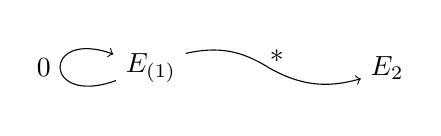
\begin{tikzpicture}
                        \node (e) at (0, 0) {$E_{(1)}$};
                        \node (e2) at (3, 0) {$E_2$};
                        \node () at (1.6, 0.1) {*};
                        \draw
                        (e) edge[out=200, in=160, distance=1cm, loop, left] node{0} (e)
                        (e) edge[bend left=22.5] (1.5, 0)
                        (1.5, 0) edge[->, bend right=22.5] (e2);
                    \end{tikzpicture}
                \end{center} 
                In the inductive case, we want to prove $P(k + 1)$, assuming $P(k)$.
                Because we're in a case where there's one or more steps, we can add a $E_1^\prime$ in our path, which is $k$ steps away from $E$.
                As we've assumed $P(k)$, it follows that there's some $E^{\prime\prime}$, such that $E_1^\prime \to^* E^{\prime\prime} \land E_2 \to^* E^{\prime\prime}$.
                This can be shown in the following diagram;
                \begin{center}
                    \begin{tikzpicture}[x=1.5cm, y=1.5cm]
                        \node (e) at (0, 0) {$E$};
                        \node (e1p) at (-1, -1) {$E_1^\prime$};
                        \node (e1) at (-2, -2) {$E_1$};
                        \node (e2) at (2, -2) {$E_2$};
                        \node (epp) at (0, -2) {$E^{\prime\prime}$};
                        \node () at (1.1, -0.9) {*};
                        \node () at (1.1, -1.9) {*};
                        \node () at (-0.4, -1.4) {*};
                        \draw
                        (e) edge[->, above] node{$k$} (e1p)
                        (e1p) edge[->] (e1)
                        (e) edge[bend right=22.5] (1, -1)
                        (1, -1) edge[->, bend left=22.5] (e2)
                        (e2) edge[bend left=22.5] (1, -2)
                        (1, -2) edge[->, bend right=22.5] (epp)
                        (e1p) edge[bend left=22.5] (-0.5, -1.5)
                        (-0.5, -1.5) edge[->, bend right=22.5] (epp);
                    \end{tikzpicture}
                \end{center}
                Now we can analyse the two cases;
                \begin{itemize}
                    \itemsep0em
                    \item $E_1^\prime = E^{\prime\prime}$
                        \subitem As we have $E_2 \to^* E^{\prime\prime}$, we get $E_2 \to^* E_1$, hence we can say $E^\prime = E_1$.
                    \item $E_1^\prime \neq E^{\prime\prime}$
                        \subitem
                            As they aren't the same, we can add a step in the path, hence $E_1^\prime \to E_1 \to^* E^{\prime\prime}$ ($E_1$ must be the next step due to determinacy).
                            Since we get $E_1 \to^* E^{\prime\prime}$, we can say $E^\prime = E^{\prime\prime}$.
                \end{itemize}
        \subsection*{30th October 2019 \hfill Lecture}
            \subsubsection*{SimpleExp}
                In this part of the lecture, our goal is to connect $\Downarrow$, and $\to^*$ for SimpleExp.
                Formally, we want to show;
                \begin{center}
                    $\forall E, n . E \Downarrow n \Leftrightarrow E \to^* n$
                \end{center}

                We first do the direction from $\Downarrow$ to $\to^*$, with the property $P(E) \triangleq \forall n . E \Downarrow n \Rightarrow E \to^* n$;
                \medskip

                There is almost no work to be done in the base case, where $E = n$, for some arbitrary $n \in \mathbb{N}$, as the big-step rule states that $n \Downarrow n$, and it takes 0 steps for $n$ to get to itself (in small-step).
                \smallskip

                For the inductive $+$ case, once again we are ignoring $\times$ as the results are quite similar, we take $E = E_1 + E_2$, with the inductive hypothesis $P(E_1) \land P(E_2)$.
                If we take some arbitrary $n$, such that $E \Downarrow n$, our rules for big-step require there to be some $n_1, n_2$ which statisfy $E_1 \Downarrow n_1$, $E_2 \Downarrow n_2$, and $n = n_1 + n_2$ (\textsc{b-add}).
                Additionally, due to our inductive hypothesis, we also get $E_1 \to^* n_1$, and also $E_2 \to^* n_2$.
                Since we have $E_1 \to^* n_1$, we can apply lemma 1, using (\textsc{s-left}), $r$ times, such that we have $E_1 + E_2 \to^* n_1 + E_2$.
                Similarly with lemma 2, using (\textsc{s-right}), we have $E_1 + E_2 \to^* n_1 + n_2$.
                Finally, due to (\textsc{s-add}), $E_1 + E_2 \to^* n$.
            \subsubsection*{While}
                In the second part of the lecture, we're revisiting the rules for the While language, which has the BNFs as follows;
                \begin{align*}
                    B \in \text{Bool} & ::= ~true~ \bnfsep ~false~ \bnfsep E = E \bnfsep E < E \bnfsep B \& B \bnfsep \neg B \bnfsep ... \\
                    E \in \text{Exp} & ::= x \bnfsep n \bnfsep E + E \bnfsep ... \\
                    C \in \text{Com} & ::= x := E \bnfsep ~if ~ B ~ then ~ C ~ else ~ C \bnfsep C;C \bnfsep ~skip~ \bnfsep ~while ~ B ~ do ~ C
                \end{align*}
                This has the following big-step rules;
                \begin{itemize}
                    \itemsep0em
                    \item \hfill
                            \axiom{$\la E, s \ra \Downarrow \la n, s^\prime \ra$}
                        \unary{$\la x := E, s \ra \Downarrow \la s^\prime [x \mapsto n] \ra$}
                        \dproof
                    \item \hfill
                            \axiom{$\la C_1, s \ra \Downarrow \la s^\prime \ra$}
                            \axiom{$\la C_2, s^\prime \ra \Downarrow \la s^{\prime\prime} \ra$}
                        \binary{$\la C_1; C_2, s \ra \Downarrow \la s^{\prime\prime} \ra$}
                        \dproof
                    \item \hfill
                            \axiom{$\la B, s \ra \Downarrow \la ~true~, s^\prime \ra$}
                            \axiom{$\la C_1, s^\prime \ra \Downarrow \la s^{\prime\prime} \ra$}
                        \binary{$\la ~if ~ B ~ then ~ C_1 ~ else ~ C_2, s \ra \Downarrow \la s^{\prime\prime} \ra$}
                        \dproof
                    \item \hfill
                            \axiom{$\la B, s \ra \Downarrow \la ~false~, s^\prime \ra$}
                            \axiom{$\la C_2, s^\prime \ra \Downarrow \la s^{\prime\prime} \ra$}
                        \binary{$\la ~if ~ B ~ then ~ C_1 ~ else ~ C_2, s \ra \Downarrow \la s^{\prime\prime} \ra$}
                        \dproof
                    \item \hfill
                            \axiom{$\la B, s \ra \Downarrow \la ~true~, s^\prime \ra$}
                            \axiom{$\la C, s^\prime \ra \Downarrow \la s^{\prime\prime} \ra$}
                            \axiom{$\la ~while ~ B ~ do ~ C, s^{\prime\prime} \Downarrow \la s^{\prime\prime\prime} \ra$}
                        \trinary{$\la ~while ~ B ~ do ~ C, s \ra \Downarrow \la s^{\prime\prime\prime} \ra$}
                        \dproof
                    \item \hfill
                            \axiom{$\la B, s \ra \Downarrow \la ~false~, s^\prime \ra$}
                        \unary{$\la ~while ~ B ~ do ~ C, s \ra \Downarrow \la s^\prime \ra$}
                        \dproof
                \end{itemize}
            After this point, there isn't any sound on the Panopto recording; the remainder of the lecture goes over heaps found in the coursework.
        \subsubsection*{6th November 2019 \hfill Tutorial}
            The lecture starts off going over questions in the coursework.
            Note that the question concerning $\neg$ can be done in a single case, with a side condition;
            \begin{center}
                    \axiom{$\la B, s, h \ra \Downarrow \la b, s^\prime, h^\prime \ra$}
                \unary{$\la \neg B, s, h \ra \Downarrow \la b^\prime, s^\prime, h^\prime \ra$}
                \dproof
                \violet{$b^\prime = \neg b$}
            \end{center}
            The next part concerns question 1 from last year's exam, which invovles the language \textsc{ForWithBreak};
            \begin{align*}
                C & ::= ~skip~ \bnfsep ~break~ \bnfsep x := E \bnfsep ~if ~ B ~ then ~ C ~ else ~ C \bnfsep ~for ~ x ~ in ~ [E, E] ~ do ~ C \bnfsep C ; C \\
                \mathcal{O} & ::= \mathcal{N} \bnfsep \mathcal{B}
            \end{align*}
            Writing out the big-step rules is too much effort; refer to the exam paper for the trees.
            \bigskip

            The ~for~ loop iterates between the values in the range, substituting $x$ for each of the values iteratively, to be used in $C$.
            The way ~break~ works is by terminating sequential commands; for example, if we had $C = ~break~; C_2$, it would evaluate to $\mathcal{B}$, and skipping the execution of $C_2$.
            However, if a ~break~ is encountered within a ~for~ loop, such that $\la C, s \ra \Downarrow_c \la \mathcal{B}, s^\prime \ra$, we terminate the loop, and then the program continues normally, such that the loop command evaluates to $\la \mathcal{N}, s^\prime \ra$.
        \subsection*{7th November 2019 \hfill Lecture}
            In a register machine, we operate on registers with idealised natural numbers (hence we don't consider physical limitations such as overflow).
            The elementary operations available to us are as follows;
            \begin{itemize}
                \itemsep0em
                \item add 1 to a register
                \item jumps
                \item test whether a register is 0 (+ conditionals)
                \item subtract 1 from a non-zero register
            \end{itemize}
            Formally, a register machine is defined 
\end{document}
